\section{Approach}
\label{sec:approach}


\begin{figure*}[th]
	\centering
	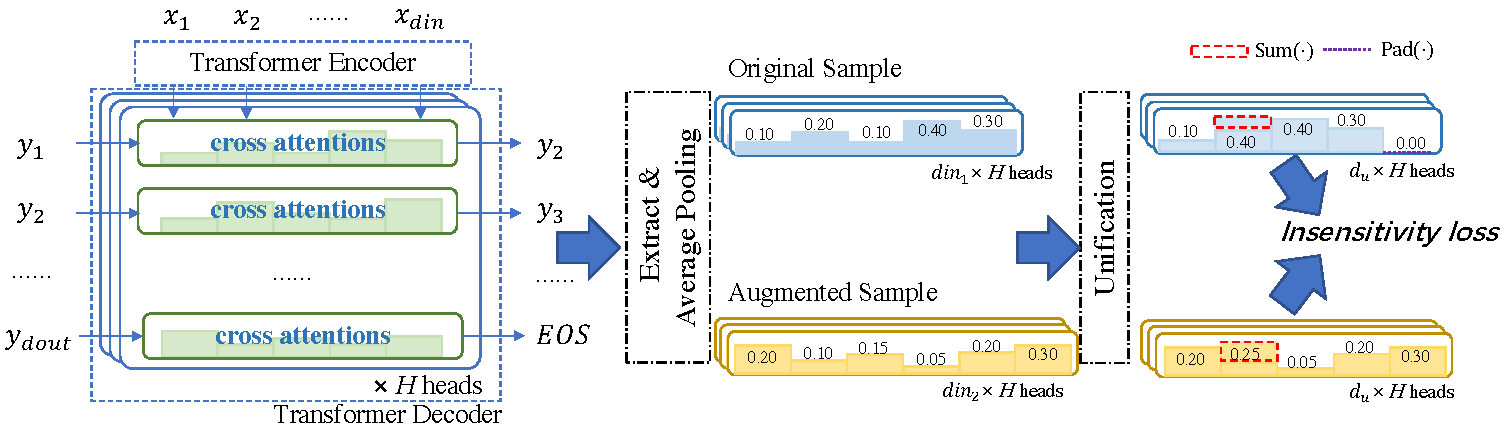
\includegraphics[scale=0.6]{insloss.pdf}
	\caption{An illustration of our Insensitivity Loss when $K=2$.
	}
	\label{fig:insloss}
\end{figure*}

We classify approaches into offline approaches and online approaches, and propose Insensitivity Loss to further reduce the sensitivity.
% two categories: in-model approaches, out-of-model approaches
\subsection{Offline Approaches}

For offline approaches, the model is fine-tuned to be more insensitive to speaker names either by data manipulations or changes in the model. No extra steps are required when using the model during the test time.
%don't need extra data processing steps during inference. 

\textbf{Augmentation (Aug)}: \citet{liu2021controllable} proposed to do data augmentation by exchanging speaker names in training samples with names from $D_{tr}$. They aim to reduce unexpected inductive bias caused by speaker names, which is similar to our goal. The model is fine-tuned with augmented training data while $D_{va}$ and $D_{te}$ remain unchanged.

\textbf{Insensitivity Loss (Ins)}: We newly propose a fine-tuning objective in this category shown in Figure~\ref{fig:insloss}, helping to reduce sensitivity with augmented data (More in ~\ref{sec:insloss}).


\subsection{Online Approaches}
\label{sec:dda}
Online approaches also need fine-tuning. The main difference is that data pre-processing steps are required before inputting into the model and post-processing after the inference during the test time. Two approaches are as follows.

\textbf{ID:} Some dataset construction work replaces speaker names with predefined IDs to avoid name bias. \{``A'', ``B''\} and \{``M'', ``F''\} are widely used for dyadic dialogues in widely-used datasets, including Mutual~\cite{cui2020mutual}, DailyDialog~\cite{li2017dailydialog}, etc. More generalized replacements is to 
normalize speakers into ``u[NUM]''~\cite{kim2019eighth} or ``\#Speaker\_[NUM]\#''~\cite{chen2021dialogsum}, which fits different number of speakers. ``[NUM]'' of a speaker is the index of its first utterance. We use ``Speaker[NUM]'' which is closer to words used during pre-training~\footnote{We didn't adopt ``\#Speaker\_[NUM]\#'' since summaries generated by models fine-tuned with such data is likely to omit ``\#''. }. Speaker names in $D_{tr}$, $D_{va}$ and $D_{te}$ are all changed.

\textbf{Frequent (Fre)}: This refers to the approach proposed in \citet{khalifa2021bag}. They use 100 male and 100 female frequent names online~\footnote{https://www.ssa.gov/oact/babynames/decades/century.html} as the pool $P$ for sampling replacements. Such a small-sized $P$ will also help to reduce the performance divergence on speaker names. Speaker names in $D_{tr}$, $D_{va}$ and $D_{te}$ are all changed as well. This approach can be further combined with the offline approaches into \textbf{FreAug} and \textbf{FreIns}.






\subsection{Insensitivity Loss}
\label{sec:insloss}

\JQ{add more intuition}
The encoder-decoder architecture is the most widely-accepted design for pre-trained generation models. At each time step, the decoder selects information to concentrate on among the encoder hidden states with the cross-attention mechanism, and predicts the current output. This soft information selection process determines the contents included in the final predictions. The intuition of Insensitivity Loss is to penalize the differences of such hidden information selection reflected by attention distributions among the same dialogue sample with different groups of speaker names. 



Mathematically, we denote the input and output of a transformer-based model as $X=\{x_1, x_2, ..., x_{din} \}$ and $Y=\{y_1, y_2, ..., y_{dout}\}$ respectively. $din$ and $dout$ represent the number of corresponding tokens.
During training, the cross attentions calculated for each output token can be collected as $CA\in R^{H\times dout \times din}$. $H$ is the number of heads for multi-head attention mechanism, which is determined by the configuration of specific pre-trained models. We apply the average pooling over the dimension of $dout$, to get the overall attention over the input tokens $\overline{CA}\in R^{H\times din}$.
% $\rm{avg}(\cdot)$

Given an original sample $\{d_i, o_i\}$, we construct $K-1$ augmented samples by replacing speaker names. The averaged attentions for all samples are $\{\overline{CA_k}\}_{k=1}^K$. Since it is a default that each sample should go through the tokenizer and truncation process before inputting to the model, $\{din_k\}_{k=1}^K$ are not guaranteed to be identical. For example, ``John'' and ``Robinson'' is tokenized into \{``John''\} and \{``Rob'', ``inson''\} by BART tokenizer. Replacing ``John'' with ``Robinson'' in $d_i$ will increase the sequence length. So, a unification function is expected before calculating the distance of these distributions. We consider two functions: \JQ{add more intuition}
\begin{itemize}
\item $\rm{Sum(\cdot)}$ sums up attention values of each token belonging to a single word of the speaker name. 
\item $\rm{Pad(\cdot)}$ pads attentions into the same length $d_u$ by concatenating zeros.
%\begin{itemize}
%	\item 
%	\item 
\end{itemize}
The unified $\{\overline{CA_k}\}_{k=1}^K$ is represented as $\{\widetilde{CA_k}\}_{k=1}^K$, where $\widetilde{CA_k}\in R^{H\times d_u}$.


Finally, the Insensitivity Loss is calculated as:
\begin{equation}
	L_{ins} = \frac{1}{C_{k}^2} \sum_{k=1}^{K}\sum_{l=1}^{K} \rm{loss}(\widetilde{CA_k}, \widetilde{CA_l})
\end{equation}
where $\rm{loss}(\cdot)$ measures the differences between each pair of attentions, and we adopt mean square error (MSE) in this paper~\footnote{The symmetric KL divergence didn't perform as good as MSE.}. This newly-introduced loss is added to the vanilla generation loss with hyper-parameter $\alpha$:
\begin{equation}
	\begin{aligned}
		L_{gen} =  \frac{1}{K}\sum_{k-1}^{K} l_{gen}(d_i^k, o_i^k) \\
		L_{total} = \alpha L_{gen} + (1-\alpha) L_{ins}
	\end{aligned}
\end{equation}
The Insensitivity Loss is only used as an auxiliary fine-tuning objective, leaving the inference time unchanged.

